\documentclass{classrep}
\usepackage[utf8]{inputenc}
\usepackage{color}
\usepackage{graphicx}
\usepackage{float}
\usepackage{environ}
\usepackage{comment}
\usepackage{amsmath}
\usepackage{amssymb}
\usepackage{amsthm}
\usepackage{longtable}
\usepackage{float}
\usepackage{lscape}
\usepackage{icomma}
{\theoremstyle{definition}
  \newtheorem{definition}{Definicja}
}

\studycycle{Informatyka, studia dzienne, I st.}
\coursesemester{VI}

\coursename{Komputerowe systemy rozpoznawania}
\courseyear{2018/2019}

\courseteacher{dr inż. Marcin Kacprowicz}
\coursegroup{poniedziałek, 14:10}

\author{
\studentinfo{Justyna Hubert}{210200} \and
\studentinfo{Karol Podlewski}{210294}
}

\title{Zadanie 2: Podsumowania lingwistyczne}
\svnurl{https://github.com/hubjust/KSR}

\begin{document}
\maketitle

\section{Cel}
Celem zadania było aplikacji desktopowej, która posiada charakter doradczy, generujący pewną ilość podsumowań lingwistycznych dla podanej bazy, a następnie przedstawia użytkownikowu wybrane - według zastosowanych miar jakości wyniki, czyli podsumowania lingwistyczne.

\section{Wprowadzenie}	
Zagadnieniem jakim zajmowaliśmy się w ramach projektu była analiza działania lingwistycznych podsumowań baz danych na zbiorach rozmytych. Zbiór rozmyty jest podstawowym pojęciem wykorzystywanym przy naszym zadaniu, zatem przytoczmy jego definicję:

\begin{definition}
Niech \(\mathcal{X}\) będzie zbiorem, którego elementy interesują
nas w sposób bezpośredni, czyli jest zbiorem klasycznym znanym z teorii mnogości (dany element przynależy do zbioru lub nie przynależy).
Wówczas \emph{zbiorem rozmytym opisanym w przestrzeni rozważań \(\mathcal{X}\)}
nazywamy każdy zbiór \(A\) postaci:
\[A = \bigcup_{x \in \mathcal{X}} \{(x,\, \mu_A(x))\},\]
gdzie \(\mu_A(x) : \mathcal{X} \to [0,\,1]\) nazywamy \emph{funkcją
przynależności do zbioru rozmytego \(A\)}.
\end{definition}

Funkcja przynależności określa w jakim stopniu dany element przynależy do zbioru. W zbiorach rozmytych zakres wartości jakie może ona przyjmować jest rozszerzony do przedziału [0,1].
W naszym projekcie skorzystaliśmy z funkcji przynależności trójkątnej oraz trapezoidalnej. Przytoczmy ich definicje:

\begin{definition}[Zbiór rozmyty o trójkątnej funkcji przynależności]
Zbiór rozmyty \(A\) typu I na uniwersum \(\mathbb{R}\) jest
\emph{liczbą rozmytą trójkątną o parametrach \(a, b, c\)} wtedy i tylko
wtedy, gdy \(a \leq b \leq c\) oraz:

\[\mu_A(x) = \begin{cases}
0                 & \mbox{gdy } x \in (-\infty,\, a], \\
(x - a) / (b - a) & \mbox{gdy } x \in (a,\, b), \\
1                 & \mbox{gdy } x = b, \\
(c - x) / (c - b) & \mbox{gdy } x \in (b,\, c), \\
0                 & \mbox{gdy } x \in [c,\, +\infty).
\end{cases}\]
\end{definition}

\vspace\baselineskip

\begin{definition}[Zbiór rozmyty o trapezoidalnej funkcji przynależności]
Zbiór rozmyty \(A\) typu I na uniwersum \(\mathbb{R}\) jest
\emph{liczbą rozmytą trapezoidalną o parametrach \(a, b, c, d\)} wtedy i tylko
wtedy, gdy \(a \leq b \leq c \leq d\) oraz:

\[\mu_A(x) = \begin{cases}
0                 & \mbox{gdy } x \in (-\infty,\, a], \\
(x - a) / (b - a) & \mbox{gdy } x \in (a,\, b), \\
1                 & \mbox{gdy } x \in [b,\, c], \\
(d - x) / (d - c) & \mbox{gdy } x \in (c,\, d), \\
0                 & \mbox{gdy } x \in [d,\, +\infty).
\end{cases}\]
\end{definition}

\vspace\baselineskip

\begin{figure}[H]
	\centering
	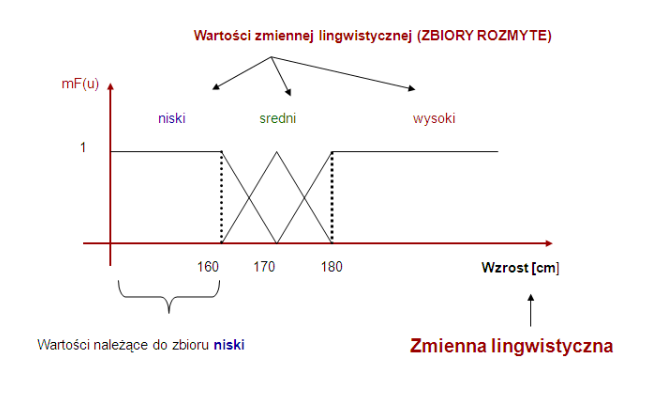
\includegraphics[width=0.9\textwidth]{{Rysunki/FunkcjaPrzynaleznosci.png}}
	\caption{Przykład funkcji przynależności - trójkątnej oraz trapezoidalnej [3]}
\end{figure}


Wyjaśnijmy także, czym jest lingwistyczne podsumowanie. Niech \(\mathcal{D}\) będzie bazą danych składającą się z \(m\)
krotek opisujących poszczególne rekordy. Przyjmijmy, że każda kolumna opisuje cechę pewnego typu. Taką cechę możemy nazwać \emph{zmienną lingwistyczną}. Może ona przyjmować konkretne wartości liczbowe lub rozmyte (np. mało/trochę/dużo/sporo). Zdefiniujmy także \(P\). Niech \(P\) będzie podmiotem podsumowania lingwistycznego (np. mężczyźni, kobiety, samochody, zawodnicy). Bardzo ważnym elementem, wykorzystywanym we wszystkich rodzajach podsumowań
lingwistycznych, jest kwantyfikator oznaczany jako \(Q\).
Przykładami kwantyfikatorów mogą być: "około 10", "ponad 70"
(kwantyfikatory absolutne - zbiory rozmyte na uniwersum \(\mathbb{R}\)) lub "większość", "znikoma część"
(kwantyfikatory relatywne - zbiory rozmyte na uniwersum \([0,\, 1]\)). Istotny dla nas będzie stopień przynależności \(P\) do \(Q\). Zdefiniujmy także sumaryzator \(S_j\). Jest to zbiór rozmyty na zbiorze wartości przyjmowanych przez \(j\)-tą kolumnę bazy danych. Np. gdyby krotki dotyczyły różnych pojazdów, a jedną ze zmiennych lingwistycznych
była ich prędkość, to sumaryzatory mogłyby mieć postać "jeździ szybko","jeździ ponad 200km/h" itp.

\vspace\baselineskip

Wykorzystując powyższe elementy można skonstruować \textbf{lingwistyczne podsumowanie
bazy danych}, czyli:
\[Q ~ P \mbox{ jest/są } S_j ~[T] ~\mbox{,}\]
gdzie \(T\) to stopień prawdziwości podsumowania.

\vspace\baselineskip

Przykład : \emph{Dużo studentów zarabia średnią krajową [0.64]}, gdzie: "dużo" to kwantyfikator, "studentów" to podmit lingwistyczny, "zarabia średnią krajową" to sumaryztaor, a "[0,64]" to stopień prawdziwości podsumowania. \newline

W celu rozszerzenie podsumowania lingwistycznego należy skorzystać ze złożonego sumaryztora. Sumę sumaryzatorów można w podsumowaniu lingwistycznym zapisać
za pomocą słowa "lub", zaś iloczyn za pomocą słowa "i".
W rezultacie \textbf{podsumowanie ze złożonym sumaryzatorem} może
mieć postać:
\[Q ~ P \mbox{ jest/są } S_1 \mbox{ i/lub } S_2 \mbox{ i/lub } \ldots \mbox{ i/lub } S_n  ~[T] ~\mbox{.}\]

\vspace\baselineskip

Przykład: \emph{Dużo studentów zarabia średnią krajową i/lub nosi okulary [0.44]}. \newline

Innym sposobem rozszerzenia pojęcia podsumowań
jest zastosowanie kwalifikatora. Kwalifikator
\(W\) jest zbiorem rozmytym na \(\mathcal{D}\),
który opisuje jakąś dodatkową właściwość. Typowe przykłady to "[osoby] które są bezrobotne",
"[osoby] które są dziećmi". \textbf{Podsumowanie
z~kwalifikatorem} ma postać:
\[Q ~ P \mbox{ mających własność } W \mbox{ ma własność } S_j ~[T] ~\mbox{.}\]

\vspace\baselineskip

Przykład: \emph{Studenci, którzy mają blond włosy zarabiają średnią krajową [028]}.\newline

Aby określić jakość naszych podsumowaniań zaimplementowaliśmy poniższe miary jakości:

\subsection{\(T_1\) -- stopień prawdziwości}

Stopień prawdziwości jest najbardziej naturalną miarą jakości podsumowania. Określa ona sumę przynależności wszystkich rozważanych krotek do sumaryzatora \(S_j\):
\[r = \sum_{i=1}^{m} \mu_{\mathrm{ce}(S_j)}(d_i) ~\mbox{,}\]
gdzie \(\mathrm{ce}(S_j)\) jest rozszerzeniem cylindrycznym
sumaryzatora \(S_j\), \(m\) liczba wszystkich krotek, a \(d_i\).
Dla kwantyfikatorów relatywnych stopnień
prawdziwości możemy zapisać jako \(T_1 = \mu_Q(\frac{r}{m})\),
zaś dla kwantyfikatorów absolutnych jako \(T_1 = \mu_Q(r)\), gdzie \(r\) jest kardynalnością. 

\subsection{\(T_2\) -- stopień nieprecyzyjności}
Dla podsumowania z \(n\) sumaryzatorami \(S_1 \ldots S_n\) możemy określić stopień nieprecyzyjności,
definiowany następującym wzorem:
\[T_2 = 1 - \left(\prod_{j=1}^{n} \mathrm{in}(S_j)\right)^{1/n} ~\mbox{.}\]
Wyrażenie \(\left(\prod_{j=1}^{n} \mathrm{in}(S_j)\right)^{1/n}\) to określa średnią geometryczna ze stopni rozmycia wykorzystanych sumaryzatorów, czyli w jakim stopniu precyzyjny jest sumaryzator. Im mniejszy nośnik zbioru rozmytego, tym wyższa jest jego precyzja.
   

\subsection{\(T_3\) -- stopień pokrycia}
Stopień pokrycia \(T_3\) jest zdefiniowany dla podsumowań z kwalifikatorami. Stopień pokrycia T3 
Dla każdego \(i=1\ldots m\) (związanego z krotką \(d_i\) z bazy
danych) możemy zdefiniować:
\[
\begin{array}{l}
t_i = \begin{cases}
1 & \mbox{gdy } \mu_{\mathrm{ce}(S_j)}(d_i) > 0 ~ \wedge ~ \mu_{W}(d_i) > 0 \\
0 & \mbox{w przeciwnym wypadku.}
\end{cases} \\
h_i = \begin{cases}
1 & \mbox{gdy } \mu_{W}(d_i) > 0 \\
0 & \mbox{w przeciwnym wypadku.}
\end{cases}
\end{array}\]

Przy powyższych oznaczeniach:
\[T_3 = \frac{\sum_{i=1}^{m} t_i}{\sum_{i=1}^{m} h_i} ~\mbox{.}\]

Reprezentuje stopień w jakim nośnik sumaryzatora pokrywa się z nośnikiem kwalifikatora.


\subsection{\(T_4\) -- stopień trafności}
Dla podsumowania z \(n\) sumaryzatorami \(S_1 \ldots S_n\)
oraz \(m\) krotkami w bazie danych możemy wprowadzić oznaczenia:
\[g_{ij} = \begin{cases}
1 & \mbox{gdy } \mu_{\mathrm{ce}(S_j)}(d_i) > 0 \\
0 & \mbox{w przeciwnym wypadku.}
\end{cases}\]
oraz
\[r_j = \frac{\sum_{i=1}^{m} g_{ij}}{m} ~\mbox{.}\]
Wówczas możemy zapisać:
\[T_4 = \left|\left \prod_{j=1}^{n} r_j \right - T_3\right| ~\mbox{.}\]

 Określa jak wiele krotek przynależy do sumaryzatora, czyli czy dane podsumowanie jest właściwe dla zestawu danych.

\subsection{\(T_5\) -- długość podsumowania}
Dla podsumowania z \(n\) sumaryzatorami \(S_1 \ldots S_n\)
miarę długości podsumowania definiujemy jako:
\[T_5 =  2 \left(\frac{1}{2}\right)^{|s|} ~\mbox{.}\]

Gdzie \(|s|\) jest ilością zbiorów rozmytych,z  których skomponowany jest sumaryzator. Określa jakość podsumowania na podstawie złożoności sumaryzatora, czyli im więcej składowych sumaryzatora złożonego, tym niższa wartość tej miary.

\subsection{\(T_6\) -- stopień nieprecyzyjności kwantyfikatora}
\(T_6\), czyli stopień nieprecyzyjności kwantyfikatora możemy zdefiniować jako:

\[T_6 = 1-\mathrm{in}(Q) ~\mbox{.}\]

Reprezentuje w jakim stopniu precyzyjny jest kwantyfikator. Im mniejszy nośnik zbioru rozmytego tym wyższa jest jego precyzja.

\subsection{\(T_7\) -- stopień liczności kwantyfikatora}
W przeciwieństwie do \(T_6\), zamiast zliczać elementy z nośnika \(Q\),
policzymy moc zbioru rozmytego:
\[T_7 = 1-\frac{\card(Q)}{\card(\mathcal{X}_Q)} ~\mbox{.}\]

Opisuje stopień precyzji kwantyfikatora, im mniejsza kardynalność kwantyfikatora tym jest on bardziej precyzyjny.

\subsection{\(T_8\) -- stopień liczności sumaryzatora}
W przypadku zastosowania sumaryzatora złożonego, podobnie jak przy poprzednich miarach, stosujemy średnią geometryczną.
Dla podsumowania z \(n\) sumaryzatorami \(S_1 \ldots S_n\):

\[T_8 = 1- \left(\prod_{j=1}^{n} \frac{\card(S_j)}{\card(\mathcal{X}_j)}\right)^{\frac{1}{n}} ~\mbox{.}\]

Opisuje stopień precyzji sumaryzatora, im mniejsza kardynalność kwantyfikatora tym jest on bardziej precyzyjny.

\subsection{\(T_9\) -- stopień nieprecyzyjności kwalifikatora}
Stopień precyzji kwalifikatora \(T_9\) jest oparty na drugiej formie podsumowań tzn.: Q obiektów będących/mających W jest/ma S, gdzie W jest reprezentowane przez zbiór rozmyty i jest kwalifikatorem. Definicja tej miary jest następująca:
\[T_9 = 1-\mathrm{in}(W) ~\mbox{.}\]

Określa w jakim stopniu precyzyjny jest kwalifikator. Im szerszy nośnik zbioru rozmytego tym niższa jest jego precyzja, gdyż bierze pod uwagę większy zakres wartości. 


\subsection{\(T_{10}\) -- stopień liczności kwalifikatora}
Stopień kardynalności kwalifikatora \(T_{10}\) definiujemy jako:
\[T_{10} = 1-\frac{\card|W|}{\card|\mathcal{X}_g|} ~\mbox{.}\]\\

Opisuje stopień precyzji kwalifikatora, im większa jest kardynalność kwalifikator tym jest on mniej precyzyjny.

\subsection{\(T_{11}\) -- długość kwalifikatora}
Długość kwalifikatora \(T_{11}\) definiujemy następująco:
\[T_{11} = 2\left(\frac{1}{2}\right)^{\card({W})} ~\mbox{.}\]

Wyznacza jakość podsumowania na podstawie złożoności kwalifikatora, Im bardziej złożony kwalifikator tym jakość podsumowania gorsza.

\vspace\baselineskip

\section{Opis implementacji}
Program został stworzony w języku C\#. Graficzny interfejs użytkownika został stworzony przy  wykorzystaniu Windows Presentation Foundation. Logika aplikacji została odseparowana od GUI. W związku z tym, zaimplementowaliśmy trzy projekty: Logic, ViewModel oraz GUI.

\subsection{Logic}
W tym projekcie zawarta została cała logika aplikacji. Odzworowany został model naszej bazy danych (\emph{FifaPlayer.cs}), zaimplementowane zostały: funkcje przynależności trójkątna (\emph{TriangularFunction.cs}) oraz trapezoidalna (\emph{TrapezoidFunction}), zmienna lingwistyczna (\emph{LinguisticVariable.cs}), kwantyfikator (\emph{Quantifier.cs}), zmienna, która "na sztywno" określa nasz kwantyfikator (np. słaby, przeciętny, dobry) w zależności od podanych danych (\emph{Variable.cs}), sumaryzator "i" (\emph{And.cs}), a także sumaryzator "lub" (\emph{Or.cs}). W projekcie logic znajduje się takża klasa (\emph{Measures.cs}), gdzie zawarliśmy wszystkie 11 miar jakości podsumowań.
 
\subsection{ViewModel}

Klasa MainViewModel przyjmuje dane wejściowe od użytkownika i reaguje na jego poczynania wywołując wybrane akcje z logiki programu oraz odpowiada za odświeżanie widoków w interfejsie graficznym

\subsection{GUI}

Projekt GUI (graphical user interface) implementuje przejrzysty oraz łatwy w obsłudze graficzny interfejs użytkownika.

\section{Materiały i metody}

\subsection{Baza danych}
Do przeprowadzenia badań i generowania konkretnych podsumowań wykorzystaliśmy bazę danych dotyczącą przechowującą statystyki piłkarzy z gry Fifa 2019 [.Składa się ona z 15397 krotek znajdujących się w tabeli z 20 różnymi kolumnami - w ramach naszego projektu skorzystaliśmy z 13. Przedstawiamy je poniżej:

\begin{itemize}
	\item Wiek - wartości z przedziału [17-45]
	\item Wzrost (cm) - wartości z przedziału [155-205]
	\item Waga (kg) - wartości z przedziału [50-11] 
	\item Tempo - wartości z przedziału [0-97]
	\item Przyspieszenie - wartości z przedziału [13-98]
	\item Prędkość - wartości z przedziału [12-97]
	\item Dribbling - wartości z przedziału [0-97]
	\item Zręczność - wartości z przedziału [14-98]
	\item Balans - wartości z przedziału [16-99]
	\item Reakcje - wartości z przedziału [30-96]
	\item Kontrola piłki - wartości z przedziału [3-97]
	\item Opanowanie - wartości z przedziału [3-97]
	\item Precyzja - wartości z przedziału [0-93]
	\item Ustawienie się - wartości z przedziału [2-95]
\end{itemize}

Każda z ww. kolumn jest typem całkowitym.

\subsection{Sumaryzatory i kwalifikatory}Poniżej zaprezentowaliśmy poszczególne sumaryzatory oraz kwalifikatory wykorzystane w naszym programie. 

\begin{table}[H]
	\centering
	\begin{tabular}{c c c c c} 
		\hline
		\textbf{Etykieta} & \textbf{a} & \textbf{b} & \textbf{c} &  \textbf{d} \\ [0.5ex] 
		\hline
		\hline 
		Bardzo młody & 17 & 17 & 18 & 20 \\ 
		Młody & 19 & 21 & 24 & 29 \\
		Dorosły & 28 & 30 & 35 & 37 \\
		Dojrzały & 36 & 40 & 45 & 45\\
		\hline
	\end{tabular}
	\caption{Przyporządkowane parametry funkcji trapezoidalnej dla wieku.}
\end{table}

\begin{table}[H]
	\centering
	\begin{tabular}{c c c c c} 
		\hline
		\textbf{Etykieta} & \textbf{a} & \textbf{b} & \textbf{c} &  \textbf{d} \\ [0.5ex] 
		\hline
		\hline 
		Bardzo niski & 155 & 155 & 160 & 162 \\ 
		Niski & 161 & 165 & 168 & 170 \\
		Przeciętny & 169 & 172 & 176 & 180 \\
		Wysoki & 179 & 182 & 186 & 192\\
		Bardzo wysoki & 191 & 196 & 205 & 205\\
		\hline
	\end{tabular}
	\caption{Przyporządkowane parametry funkcji trapezoidalnej dla wzrostu.}
\end{table}

\begin{table}[H]
	\centering
	\begin{tabular}{c c c c c} 
		\hline
		\textbf{Etykieta} & \textbf{a} & \textbf{b} & \textbf{c} &  \textbf{d} \\ [0.5ex] 
		\hline
		\hline 
		Niska & 50 & 59 & 66 & 73 \\ 
		Standardowa & 72 & 77 & 79 & 84 \\
		Postawna & 83 & 86 & 89 & 91 \\
		Ciężka & 90 & 98 & 110 & 110\\
		\hline
	\end{tabular}
	\caption{Przyporządkowane parametry funkcji trapezoidalnej dla wzrostu.}
\end{table}

\begin{table}[H]
	\centering
	\begin{tabular}{c c c c c} 
		\hline
		\textbf{Etykieta} & \textbf{a} & \textbf{b} & \textbf{c} &  \textbf{d} \\ [0.5ex] 
		\hline
		\hline 
		Niskie & 0 & 15 & 27 & 35 \\ 
		Średnie & 33 & 46 & 58 & 66 \\
		Wysokie & 65 & 79 & 88 & 97 \\
		\hline
	\end{tabular}
	\caption{Przyporządkowane parametry funkcji trapezoidalnej dla tempa.}
\end{table}

\begin{table}[H]
	\centering
	\begin{tabular}{c c c c c} 
		\hline
		\textbf{Etykieta} & \textbf{a} & \textbf{b} & \textbf{c} &  \textbf{d} \\ [0.5ex] 
		\hline
		\hline 
		Słabe & 13 & 25 & 29 & 35 \\ 
		Przieciętne & 33 & 46 & 58 & 66 \\
		Dobre & 65 & 79 & 88 & 98 \\
		\hline
	\end{tabular}
	\caption{Przyporządkowane parametry funkcji trapezoidalnej dla przyspieszenia.}
\end{table}

\begin{table}[H]
	\centering
	\begin{tabular}{c c c c c} 
		\hline
		\textbf{Etykieta} & \textbf{a} & \textbf{b} & \textbf{c} &  \textbf{d} \\ [0.5ex] 
		\hline
		\hline 
		Słaba & 12 & 25 & 29 & 35 \\ 
		Przieciętna & 33 & 46 & 58 & 69 \\
		Dobra & 65 & 79 & 88 & 97 \\
		\hline
	\end{tabular}
	\caption{Przyporządkowane parametry funkcji trapezoidalnej dla prędkości.}
\end{table}

\begin{table}[H]
	\centering
	\begin{tabular}{c c c c c} 
		\hline
		\textbf{Etykieta} & \textbf{a} & \textbf{b} & \textbf{c} &  \textbf{d} \\ [0.5ex] 
		\hline
		\hline 
		Słaby & 0 & 15 & 27 & 37 \\ 
		Przieciętny & 36 & 46 & 58 & 66 \\
		Dobry & 67 & 79 & 88 & 97 \\
		\hline
	\end{tabular}
	\caption{Przyporządkowane parametry funkcji trapezoidalnej dla dribblingu.}
\end{table}

\begin{table}[H]
	\centering
	\begin{tabular}{c c c c c} 
		\hline
		\textbf{Etykieta} & \textbf{a} & \textbf{b} & \textbf{c} &  \textbf{d} \\ [0.5ex] 
		\hline
		\hline 
		Słaba & 14 & 21 & 27 & 35 \\ 
		Przieciętna & 33 & 46 & 58 & 69 \\
		Dobra & 67 & 79 & 88 & 98 \\
		\hline
	\end{tabular}
	\caption{Przyporządkowane parametry funkcji trapezoidalnej dla zręczności.}
\end{table}

\begin{table}[H]
	\centering
	\begin{tabular}{c c c c c} 
		\hline
		\textbf{Etykieta} & \textbf{a} & \textbf{b} & \textbf{c} &  \textbf{d} \\ [0.5ex] 
		\hline
		\hline 
		Słaby & 16 & 21 & 29 & 35 \\ 
		Przieciętny & 38 & 46 & 58 & 72 \\
		Dobry & 71 & 79 & 88 & 99 \\
		\hline
	\end{tabular}
	\caption{Przyporządkowane parametry funkcji trapezoidalnej dla balansu.}
\end{table}

\begin{table}[H]
	\centering
	\begin{tabular}{c c c c c} 
		\hline
		\textbf{Etykieta} & \textbf{a} & \textbf{b} & \textbf{c} &  \textbf{d} \\ [0.5ex] 
		\hline
		\hline 
		Słabe & 30 & 37 & 43 & 47 \\ 
		Przeciętne & 46 & 59 & 66 & 72 \\
		Szybkie & 71 & 79 & 88 & 96 \\
		\hline
	\end{tabular}
	\caption{Przyporządkowane parametry funkcji trapezoidalnej dla reakcji.}
\end{table}

\begin{table}[H]
	\centering
	\begin{tabular}{c c c c c} 
		\hline
		\textbf{Etykieta} & \textbf{a} & \textbf{b} & \textbf{c} &  \textbf{d} \\ [0.5ex] 
		\hline
		\hline 
		Słaba & 3 & 14 & 23 & 26 \\ 
		Przieciętna & 25 & 39 & 48 & 57 \\
		Dobra & 56 & 63 & 69 & 75 \\
		Bardzo dobra & 74 & 81 & 88 & 99 \\
		\hline
	\end{tabular}
	\caption{Przyporządkowane parametry funkcji trapezoidalnej dla kontroli piłki.}
\end{table}

\begin{table}[H]
	\centering
	\begin{tabular}{c c c c c} 
		\hline
		\textbf{Etykieta} & \textbf{a} & \textbf{b} & \textbf{c} &  \textbf{d} \\ [0.5ex] 
		\hline
		\hline 
		Słabe & 3 & 15 & 24 & 32 \\ 
		Zadowalające & 31 & 44 & 57 & 66 \\
		Bardzo dobre & 65 & 75 & 88 & 97 \\
		\hline
	\end{tabular}
	\caption{Przyporządkowane parametry funkcji trapezoidalnej dla opanowania.}
\end{table}

\begin{table}[H]
	\centering
	\begin{tabular}{c c c c c} 
		\hline
		\textbf{Etykieta} & \textbf{a} & \textbf{b} & \textbf{c} &  \textbf{d} \\ [0.5ex] 
		\hline
		\hline 
		Słaba & 3 & 15 & 24 & 32 \\ 
		Przeciętna & 31 & 44 & 57 & 66 \\
		Dobra & 65 & 75 & 88 & 97 \\
		\hline
	\end{tabular}
	\caption{Przyporządkowane parametry funkcji trapezoidalnej dla celności.}
\end{table}

\begin{table}[H]
	\centering
	\begin{tabular}{c c c c c} 
		\hline
		\textbf{Etykieta} & \textbf{a} & \textbf{b} & \textbf{c} &  \textbf{d} \\ [0.5ex] 
		\hline
		\hline 
		Słabe & 3 & 15 & 24 & 32 \\ 
		Przeciętne & 31 & 44 & 57 & 66 \\
		Dobre & 65 & 75 & 88 & 97 \\
		\hline
	\end{tabular}
	\caption{Przyporządkowane parametry funkcji trapezoidalnej dla ustawiania się.}
\end{table}

\subsection{Kwantyfikatory}
Kwantyfikatory podzieliliśmy na względne i absolutne . Przedstawiamy je poniżej:

\begin{table}[H]
	\centering
	\begin{tabular}{c c c c c c} 
		\hline
		\textbf{Etykieta} & \textbf{Funkcja przynależności} & \textbf{a} & \textbf{b} & \textbf{c} &  \textbf{d} \\ [0.5ex] 
		\hline
		\hline 
		Żaden & Trójkątna & 0 & 0 & 0.1 & - \\ 
		Mniej niż ćwierć & Trapezoidalna & 0 & 0 & 0.2 & 0.25 \\
		Około jedna trzecia & Trójkątna & 0.23 & 0.33 & 0.43 & - \\
		Około połowa & Trójkątna & 0.4 & 0.5 & 0.6 & - \\
		Około dwie trzecie & Trójkątna & 0.56 & 0.66 & 0.76 & - \\
		Większość & Trójkątna & 0.73 & 0.83 & 0.93 & - \\
		Prawie każdy & Trójkątna & 0.85 & 0.9 & 1.05 & - \\
		\hline
	\end{tabular}
	\caption{Przyporządkowane parametry dla kwantyfikatora względnego.}
\end{table}
\begin{table}[H]
	\centering
	\begin{tabular}{c c c c c c} 
		\hline
		\textbf{Etykieta} & \textbf{Funkcja przynależności} & \textbf{a} & \textbf{b} & \textbf{c} &  \textbf{d} \\ [0.5ex] 
		\hline
		\hline 
		Mniej niż 1000 & Trapezoidalna & 0 & 0 & 900 & 1000 \\ 
		Około 4000 & Trójkątna & 3000 & 4000 & 5000 & - \\
		Około 8000 & Trójkątna & 7000 & 8000 & 9000 & - \\
		Więcej niż 1000 & Trapezoidalna & 9000 & 9990 & 10000 & 20000 \\
		\hline
	\end{tabular}
	\caption{Przyporządkowane parametry dla kwantyfikatora absolutnego.}
\end{table}


\section{Wyniki}

Poniższej umieszczone tabele oraz wykresy są wynikami przeprowadzonych przez nas eksperymentów.

\subsection{Wpływ liczby k sąsiadów oraz wyboru metryki na klasyfikację}


\section{Dyskusja}

\subsection{Wpływ liczby k sąsiadów oraz wyboru metryki na klasyfikację}
W przypadku wszystkich trzech sposobów ekstrakcji, metryka Euklidesowa oraz metryka uliczna osiągają bardzo podobne wyniki i nie jesteśmy w stanie stwierdzić, która z nich wykazuje lepszą skuteczność. Metryka Czebyszewa charakteryzuje się zdecydowanie słabszą zdolnością do klasyfikacji. Osiąga niższe wyniki, niż dwie wcześniej wspomniane metryki.
 \newline

W przypadku pierwszego i drugiego sposobu ekstrakcji cech dla kategorii topics i places, zauważyliśmy, że wraz ze wzrostem liczby k sąsiadów zwiększała się także skuteczność. Najsłabsze wyniki osiągane były dla k równego 2. Jeśli zaś chodzi o kategorię authors, najwyższa skuteczność wykazywała mała liczba k sąsiadów (od 2 do 3). Wyraźny spadek wyników zaobserwowaliśmy, gdy k równało się 10. Podczas eksperymentu trzeciego sposobu ekstrakcji cech zauważyliśmy bardzo zmienną skuteczność w przypadku zmiany liczby k sąsiadów w zależności od wybranych kategorii. Kategoria places osiąga najsłabsze wyniki przy małej liczbie sąsiadów, z kolei kategoria topics najlepsze. Zauważyliśmy, że najwyższe wyniki w kategorii authors osiągane są przy liczbie sąsiadów równej 7 oraz 10. 


\subsection{Wpływ podziału tekstów na zbiory treningowe i testowe na klasyfikację}
W przeważającej większości najwyższe wyniki osiągane były przy 80\% zbioru treningowego. Tylko w jednym przypadku użycie 40\% zbioru treningowego pozwoliło osiągnąć najwyższą skuteczności (pierwszy sposób ekstrakcji, kategoria topics). Zazwyczaj jednak ten dobór procentowy okazywał się być najsłabszym ze względu na niedouczenie. 
\newline

\subsection{Wpływ konkretnych cech na klasyfikację}
Podczas klasyfikacji dla kategorii topics, zauważyliśmy, że liczba słów oraz liczba słów, których długość nie przekracza 3 znaków mają negatywny wpływ na osiąganą skuteczność. Świadczyć może o tym fakt, iż bez ww. cech osiągnęliśmy najwyższą skuteczność. Dużo ważniejsze okazały się cechy związane z unikalnością słów oraz wielkimi literami. \newline

Podczas klasyfikacji dla kategorii authors najważniejsza okazała się cecha odpowiadająca za liczbę unikalnych słów. Bez niej skuteczność spadła z 71\% na 47\%. Podobnie jak w przypadku kategorii topics, cechy sprawdzające liczbę słów oraz liczbę krótkich słów osłabiały nasze wyniki - dzięki wyłączeniu ich, uzyskaliśmy wyższe wyniki niż w przypadku wszystkich cech. 

	
\section{Wnioski}
\begin{itemize}
	\item Liczba k sąsiadów ma spory wpływ na skuteczność klasyfikacji, jednak nie ma jednej, optymalnej wartości - zmiana metryki, podziału zbiorów czy klasyfikowanych kategorii może spowodować obniżenie wyników dla stałego k.
	\item Dla mniejszych zbiorów tekstowych lepiej sprawdzają się mniejsze wartości k sąsiadów, dla większych - wyższe wartości.
	\item Metryka Czebyszewa nie powinna być wykorzystywana w klasyfikacji tekstów, gdyż osiąga bardzo słabe wyniki.
	\item Istotny jest podział tekstów na zbiory testowe oraz treningowe. W przypadku zbyt małego zbioru treningowego osiągamy zjawisko niedouczenia, w przypadku zbyt dużego - przeuczenia.
	\item Cechy odpowiedzialne za liczbę słów oraz liczbę krótkich słów (do 3 znaków)  nie sprawdzają się przy klasyfikacji tekstów.
	\item Wektor cech powinien się składać z przynajmniej kilku cech, żeby osiągnąć większą skuteczność.
\end{itemize}

	

\begin{thebibliography}{}
\bibitem{adam}
Methods for the linguistic summarization of data - aplications of fuzzy sets and their extensions, Adam Niewiadomski, Akademicka Oficyna Wydawnicza EXIT, Warszawa 2008
\bibitem{ZbiorRozmyty}
http://www.cs.put.poznan.pl/amichalski/si.dzienne/AI7.new.fuzzy.b&w.pdf
\bibitem{FunkcjaPrzynaleznosci}
http://home.agh.edu.pl/~mrzyglod/iw/iw_pliki/iw-is-L2-2017-2018.pdf
\bibitem{BazaDanych}
https://www.kaggle.com/aishwarya1992/fifa-19-player-database
\end{thebibliography}
\end{document}
